\documentclass{beamer}

\usepackage{amsmath}

\usepackage{tikz}
\usetikzlibrary{tikzmark}
\usetikzlibrary{decorations.pathreplacing}
\usetikzlibrary{fit}
\usetikzlibrary{graphs}

\title{All for one and none forall: Compiling polymorphic relations without monomorphization}
\author{Dmitri Volkov, Yafei Yang, Chung-chieh Shan}
\date{2026 August 24}

\begin{document}

\begin{frame}
	\titlepage
\end{frame}

\begin{frame}

	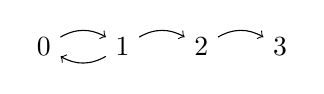
\begin{tikzpicture}
		\graph[edges={bend left}] { 0 -> 1 -> 2 -> 3, 1 -> 0 };
	\end{tikzpicture}

	\begin{align*}
		\begin{aligned}
			& \texttt{(defrel (graph} \\
			&\quad \texttt{(from : (Num 4)) (to : (Num 4)))} \\
			&\quad \texttt{(disj} \\
			&\quad\quad \texttt{(conj (== from 0) (== to 1))} \\
			&\quad\quad \texttt{(conj (== from 1) (== to 2))} \\
			&\quad\quad \texttt{(conj (== from 1) (== to 0))} \\
			&\quad\quad \texttt{(conj (== from 2) (== to 3))))} \\
		\end{aligned}
		&&
		\begin{matrix}
			& & \text{to} \\
			& & \begin{matrix} 0 & 1 & 2 & 3 \end{matrix} \\
			\text{from} & \begin{matrix} 0 \\ 1 \\ 2 \\ 3 \end{matrix} &
			\begin{bmatrix}
				0 & 1 & 0 & 0 \\
				1 & 0 & 1 & 0 \\
				0 & 0 & 0 & 1 \\
				0 & 0 & 0 & 0 \\
			\end{bmatrix}
		\end{matrix}
	\end{align*}

	Can represent the graph as a relation or as an adjacency matrix.\\
	semiringKanren computes matrices for arbitrary relations!

\end{frame}

\begin{frame}

	semiringKanren values are drawn from algebraic data types.
	
	Let \(\texttt{x}\) be a value of type \(\alpha\), and \(\texttt{y}\) be a value of type \(\beta\).

	We notate this as:
	\begin{align*}
		\texttt{x} : \alpha \\
		\texttt{y} : \beta \\
	\end{align*}

	semiringKanren has the following value constructors and corresponding types:
	\begin{itemize}
		\item \(\texttt{sole} : \texttt{Unit}\)
		\item \(\texttt{(left x)} : \texttt{(Sum \(\alpha\) \(\beta\))}\)
		\item \(\texttt{(right y)} : \texttt{(Sum \(\alpha\) \(\beta\))}\)
	\end{itemize}

	(semiringKanren also has product types)

\end{frame}

\begin{frame}
	
	We abbreviate types by their size, and index values.

	\begin{align*}
		\texttt{(Sum Unit (Sum Unit Unit))} &\mapsto \mathtt{3} \\
		\texttt{(left sole)} &\mapsto \mathtt{0_3} \\
		\texttt{(right (left sole))} &\mapsto \mathtt{1_3} \\
		\texttt{(right (right sole))} &\mapsto \mathtt{2_3} \\
	\end{align*}

\end{frame}

\begin{frame}

	Relations denote arrays; entries correspond to argument values, and hold weights.
	Here, weight 1 denotes success and weight 0 denotes failure.

	\begin{align*}
		& \texttt{(defrel (R (x : \(3\)))} \\
		& \quad \texttt{(== x \(\mathtt{0_3}\)))} \\
	\end{align*}

	\begin{align*}
		\begin{matrix}
			\begin{matrix} \mathtt{0_3} & \mathtt{1_3} & \mathtt{2_3} \end{matrix} \\
			\begin{bmatrix} 1 & 0 & 0 \end{bmatrix}
		\end{matrix}
	\end{align*}

	(semiringKanren supports computing over weights drawn from any commutative semiring)

\end{frame}

\begin{frame}

	\(\texttt{disj}\) is addition.

	\begin{align*}
		& \texttt{(defrel (R (x : \(3\)))} \\
		& \quad \texttt{(disj} \\
		& \quad\quad \texttt{(== x \(\mathtt{0_3}\))} \\
		& \quad\quad \texttt{(== x \(\mathtt{2_3}\))))} \\
	\end{align*}

	\begin{align*}
		\begin{bmatrix} 1 & 0 & 0 \end{bmatrix} + \begin{bmatrix} 0 & 0 & 1 \end{bmatrix} \\
		\begin{matrix}
			\begin{matrix} \mathtt{0_3} & \mathtt{1_3} & \mathtt{2_3} \end{matrix} \\
			\begin{bmatrix} 1 & 0 & 1 \end{bmatrix}
		\end{matrix}
	\end{align*}

\end{frame}

\begin{frame}

	\(\texttt{conj}\) is multiplication.

	\begin{align*}
		& \texttt{(defrel (R (x : \(3\)))} \\
		& \quad \texttt{(conj} \\
		& \quad\quad \texttt{(== x \(\mathtt{0_3}\))} \\
		& \quad\quad \texttt{(== x \(\mathtt{2_3}\))))} \\
	\end{align*}

	\begin{align*}
		\begin{bmatrix} 1 & 0 & 0 \end{bmatrix} * \begin{bmatrix} 0 & 0 & 1 \end{bmatrix} \\
		\begin{matrix}
			\begin{matrix} \mathtt{0_3} & \mathtt{1_3} & \mathtt{2_3} \end{matrix} \\
			\begin{bmatrix} 0 & 0 & 0 \end{bmatrix}
		\end{matrix}
	\end{align*}

\end{frame}

\begin{frame}

	Multi-argument relations denote multidimensional arrays.

	\begin{align*}
		& \texttt{(defrel (R (x : 3) (y : 3)} \\
		& \quad \texttt{(== x y)))} \\
	\end{align*}
	\begin{align*}
		\begin{matrix}
			&
			\begin{matrix} \mathtt{0_3} & \mathtt{1_3} & \mathtt{2_3} \end{matrix}
			\\
			\begin{matrix} \mathtt{0_3} \\ \mathtt{1_3} \\ \mathtt{2_3} \end{matrix}
			&
			\begin{bmatrix}
				1 & 0 & 0 \\
				0 & 1 & 0 \\
				0 & 0 & 1 \\
			\end{bmatrix}
		\end{matrix}
	\end{align*}

\end{frame}


\begin{frame}

	\begin{align*}
		\begin{bmatrix}
			0 & 0 & 0 & 1 & 0 & 0 \\
			0 & 0 & 0 & 0 & 1 & 0 \\
			0 & 0 & 0 & 0 & 0 & 1 \\
			1 & 0 & 0 & 0 & 0 & 0 \\
			0 & 1 & 0 & 0 & 0 & 0 \\
			0 & 0 & \tikzmarknode{sumswapa3b3-52}{1} & 0 & 0 & 0 \\
		\end{bmatrix}
		&&
		\begin{bmatrix}
			0 & 0 & 0 & 0 & 1 & 0 & 0 \\
			0 & 0 & 0 & 0 & 0 & 1 & 0 \\
			0 & 0 & 0 & 0 & 0 & 0 & 1 \\
			1 & 0 & 0 & 0 & 0 & 0 & 0 \\
			0 & 1 & 0 & 0 & 0 & 0 & 0 \\
			0 & 0 & 1 & 0 & 0 & 0 & 0 \\
			0 & 0 & 0 & \tikzmarknode{sumswapa3b4-63}{1} & 0 & 0 & 0 \\
		\end{bmatrix}
	\end{align*}

	\begin{align*}
		\begin{aligned}
		x &\mapsto \tikzmarknode{sumswapa3b3-52vals}{} \texttt{(\tikzmarknode{sumswapa3b3xright}{right} \tikzmarknode{sumswapa3b3xrighthole}{\(\underline{\mathtt{2_3}}\))}} \\
		y &\mapsto \texttt{(\tikzmarknode{sumswapa3b3yleft}{left} \tikzmarknode{sumswapa3b3ylefthole}{\(\underline{\mathtt{2_3}}\))}}
		\end{aligned}
		&&
		\begin{aligned}
		x &\mapsto \tikzmarknode{sumswapa3b4-63vals}{} \texttt{(\tikzmarknode{sumswapa3b4xright}{right} \tikzmarknode{sumswapa3b4xrighthole}{\(\underline{\mathtt{3_4}}\))}} \\
		y &\mapsto \texttt{(\tikzmarknode{sumswapa3b4yleft}{left} \tikzmarknode{sumswapa3b4ylefthole}{\(\underline{\mathtt{3_4}}\))}}
		\end{aligned}
	\end{align*}
	
	\begin{center}
		\tikzmarknode{xisright}{\(x\) is \texttt{(right \(\dots\))}}
		\hfill
		\tikzmarknode{yisleft}{\(y\) is \texttt{(left \(\dots\))}}
		\hfill
		\tikzmarknode{betasequal}{\(\beta\)-typed parts equal}
	\end{center}

	\begin{tikzpicture}[remember picture,overlay]

		% \node[draw=red, rectangle, fit=()] {};

		\draw[->, shorten <=1mm, shorten >=3mm] (sumswapa3b3-52) to (sumswapa3b3-52vals);
		\draw[->, shorten <=1mm, shorten >=3mm] (sumswapa3b4-63) to (sumswapa3b4-63vals);

		\draw[->] (sumswapa3b3xright.north) to[bend right=115] (xisright);
		\draw[->] (sumswapa3b4xright.north) to[bend right, in=-90] (xisright);

		\draw[->] ([yshift=-1mm]sumswapa3b3yleft.south) to (yisleft);
		\draw[->] ([yshift=-1mm]sumswapa3b4yleft.south) to (yisleft);

		\draw[decorate, decoration=brace] (sumswapa3b3xrighthole.north east) to node(2eq2)[right] {\(\mathtt{2_3} = \mathtt{2_3}\)} (sumswapa3b3xrighthole.east |- sumswapa3b3ylefthole.south);
		\draw[decorate, decoration=brace] (sumswapa3b4xrighthole.north east) to node(3eq3)[right] {\(\mathtt{3_4} = \mathtt{3_4}\)} (sumswapa3b4xrighthole.east |- sumswapa3b4ylefthole.south);

		\draw[->] (2eq2.south) -- (betasequal);
		\draw[->] (3eq3.south) -- (betasequal);
	\end{tikzpicture}

\end{frame}

\end{document}
